\documentclass[letterpaper,11pt]{article}

\usepackage{latexsym}
\usepackage[empty]{fullpage}
\usepackage{titlesec}
\usepackage{marvosym}
\usepackage[usenames,dvipsnames]{color}
\usepackage{verbatim}
\usepackage{enumitem}
\usepackage[hidelinks]{hyperref}
\usepackage{fancyhdr}
\usepackage[english]{babel}
\usepackage{tabularx}
\usepackage{fontawesome5}
\usepackage{multicol}
\setlength{\multicolsep}{-3.0pt}
\setlength{\columnsep}{-1pt}
\input{glyphtounicode}

%new packages

\usepackage{fontenc}
\usepackage{amsmath}
\usepackage{amssymb}
\usepackage{graphicx}



%----------FONT OPTIONS----------

\pagestyle{fancy}
\fancyhf{} % clear all header and footer fields
\fancyfoot{}
\renewcommand{\headrulewidth}{0pt}
\renewcommand{\footrulewidth}{0pt}

% Adjust margins
\addtolength{\oddsidemargin}{-0.6in}
\addtolength{\evensidemargin}{-0.5in}
\addtolength{\textwidth}{1.19in}
\addtolength{\topmargin}{-.7in}
\addtolength{\textheight}{1.4in}

\urlstyle{same}

\raggedbottom
\raggedright
\setlength{\tabcolsep}{0in}

% Sections formatting
\titleformat{\section}{
  \vspace{-4pt}\scshape\raggedright\large\bfseries
}{}{0em}{}[\color{black}\titlerule \vspace{-5pt}]



% Ensure that generate pdf is machine readable/ATS parsable
\pdfgentounicode=1

%-------------------------
% Custom commands
\newcommand{\resumeItem}[1]{
  \item\small{
    {#1 \vspace{-2pt}}
  }
}

\newcommand{\classesList}[4]{
    \item\small{
        {#1 #2 #3 #4 \vspace{-2pt}}
  }
}

\newcommand{\resumeSubheading}[4]{
  \vspace{-2pt}\item
    \begin{tabular*}{1.0\textwidth}[t]{l@{\extracolsep{\fill}}r}
      \textbf{#1} & \textbf{\small #2} \\
      \textit{\small#3} & \textit{\small #4} \\
    \end{tabular*}\vspace{-7pt}
}

\newcommand{\resumeSubSubheading}[2]{
    \item
    \begin{tabular*}{0.97\textwidth}{l@{\extracolsep{\fill}}r}
      \textit{\small#1} & \textit{\small #2} \\
    \end{tabular*}\vspace{-7pt}
}

\newcommand{\resumeProjectHeading}[2]{
    \item
    \begin{tabular*}{1.001\textwidth}{l@{\extracolsep{\fill}}r}
      \small#1 & \textbf{\small #2}\\
    \end{tabular*}\vspace{-7pt}
}


\newcommand{\resumeSubItem}[1]{\resumeItem{#1}\vspace{-4pt}}

\renewcommand\labelitemi{$\vcenter{\hbox{\tiny$\bullet$}}$}
\renewcommand\labelitemii{$\vcenter{\hbox{\tiny$\bullet$}}$}

\newcommand{\resumeSubHeadingListStart}{\begin{itemize}[leftmargin=0.0in, label={}]}
\newcommand{\resumeSubHeadingListEnd}{\end{itemize}}
\newcommand{\resumeItemListStart}{\begin{itemize}}
\newcommand{\resumeItemListEnd}{\end{itemize}\vspace{-5pt}}


\begin{document}
\fontfamily{cmr}\selectfont
\begin{center}
\parbox{3.0cm}{%
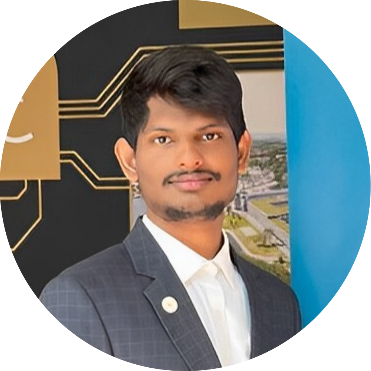
\includegraphics[width=2.7cm,clip]{images/resume_pic_m.png}}
}
\parbox{\dimexpr\linewidth-3.8cm\relax}{
\vspace{-20pt}
\begin{tabularx}{\linewidth}{L r} \\
    {\Huge \scshape  Venkata Sai Yakkshit Reddy Asodi}~
    \href{https://www.cedzlabs.com/yakkshit}{\vspace{1pt}}\\
      Berlin, Germany. \\ \vspace{1pt}
     \small \raisebox{-0.1\height}\faPhone\ +91 8179936156 ~ \href{mailto:saiyakkshit2001@gmail.com}{\raisebox{-0.2\height}\faEnvelope\  {saiyakkshit2001@gmail.com}} ~ 
    \href{https://linkedin.com/in/yakkshit/}{\raisebox{-0.2\height}\faLinkedin\ {yakkshit}}  ~
    \href{https://yakkshit.com/}{\raisebox{-0.2\height}\faGlobe\ {yakkshit.com}}  ~
    \href{https://github.com/yakkshit}{\raisebox{-0.2\height}\faGithub{ yakkshit}}
    \vspace{-8pt}
\end{tabularx}
}
\end{center}

\vspace{-23pt}
%-----------SUMMARY-----------
\href{https://www.yakkshit.com/#details}{\section{Summary \faLink}
Innovative AI Engineer with expertise in LLMs, RAG systems, and document processing pipelines. Proven track record of building and deploying production-ready AI solutions in fast-paced startup environments. Passionate about leveraging cutting-edge AI to simplify complex bureaucratic processes and create user-friendly automated solutions. Strong background in full-stack development enabling end-to-end AI system implementation.}

%-----------TECHNICAL SKILLS-----------
\section{\href{https://www.linkedin.com/in/yakkshit/details/skills/}{Technical Skills} \faLink}
\begin{itemize}[leftmargin=0.15in, label={}]
\small{\item{
\textbf{AI/ML - }{LLMs, RAG, Langchain, Hugging Face, Document AI, Recommendation Systems} \\
\textbf{Languages - }{Python, JavaScript, SQL, HTML5, CSS3} \\
\textbf{Frameworks - }{FastAPI, React, Jupyter, PyTorch, TensorFlow} \\
\textbf{Cloud \& Tools - }{AWS, Azure, Docker, Kubernetes, Git, MLflow} \\
}}
\end{itemize}
\vspace{-10pt}

%-----------EXPERIENCE-----------
\section{Experience \faLinkedin}

\resumeSubHeadingListStart

\resumeSubheading
{\large Circleup AG \faBuilding}{December 2023 -- July 2024}
{Lead AI/ML Engineer}{\faMapMarker \hspace{0.1cm} Zurich, Switzerland}\\
\vspace{10pt}
\textbf{Responsibilities:}
\resumeItemListStart
\vspace{-10pt}
\resumeItem{Architected and implemented production-grade RAG systems and LLM pipelines for automated document processing and information extraction, achieving 85\% reduction in manual processing time. Built and deployed custom agents for document analysis and form filling.}
\resumeItem{Developed scalable recommendation engines using FastAPI and Azure AI services, processing 100k+ documents monthly. Implemented comprehensive evaluation frameworks for continuous monitoring of LLM performance and accuracy.}
\resumeItemListEnd
\vspace{-3pt}
\textbf{Environment:}\emph{Python, FastAPI, Azure AI, LangChain, Docker, Jupyter, MLflow}

\resumeSubheading
{Cedzlabs \faBuilding}{March 2023 -- July 2024}
{AI Solutions Engineer}{\faMapMarker \hspace{0.1cm} India}\\
\vspace{10pt}
\textbf{Responsibilities:}
\vspace{-10pt}
\resumeItemListStart
\resumeItem{Built end-to-end document processing systems using transformer models and custom RAG pipelines, reducing processing time by 70\%. Developed and deployed AI agents for automated data extraction and form filling, handling complex document structures and varying formats.}
\resumeItemListEnd
\vspace{-3pt}
\textbf{Environment:}\emph{Python, Hugging Face, AWS, FastAPI, Docker, LLMs}

%-----------PROJECTS-----------
\section{Projects \faGithub}
\vspace{-5pt}
\resumeSubHeadingListStart

\resumeProjectHeading
{\textbf{\href{https://ui.cedzlabs.com/resume}{Intelligent Document Processing System}} $|$ \emph{Azure AI, FastAPI, RAG}}{2023-2024}\\
\vspace{6pt}
\textbf{Description:}
\vspace{-5pt}
\resumeItemListStart
\resumeItem{Developed a comprehensive document processing platform using RAG and LLM-powered agents. Built custom pipelines for document understanding, information extraction, and automated form filling. Implemented sophisticated recommendation engine for document classification and routing. Deployed on Azure with high-availability architecture processing 10,000+ documents daily.}
\resumeItemListEnd
\vspace{4pt}
\textbf{Tools:}\emph{Python, FastAPI, Azure AI, LangChain, Docker, Kubernetes}
\vspace{-10pt}

\resumeProjectHeading
{\textbf{Tender Matching Engine} $|$ \emph{AWS, LLMs, RAG}}{2023}\\
\vspace{6pt}
\textbf{Description:}
\vspace{-5pt}
\resumeItemListStart
\resumeItem{Built an AI-powered system for matching companies with relevant government tenders using custom RAG pipelines and recommendation algorithms. Implemented automated tender document analysis and requirement extraction, improving matching accuracy by 65\%.}
\resumeItemListEnd
\vspace{4pt}
\textbf{Tools:}\emph{Python, AWS, Hugging Face, FastAPI, Docker}
\vspace{-12pt}

%-----------ACHIEVEMENTS---------------
\section{Achievements / Contributions}
\resumeSubHeadingListStart
\resumeItemListStart
\resumeItem{Developed open-source RAG framework for document processing with 1000+ GitHub stars.}
\resumeItem{Led workshops on implementing production-grade LLM systems and document processing pipelines.}
\resumeItem{Published technical blog posts on optimizing RAG systems for enterprise document processing.}
\resumeItemListEnd

\resumeSubHeadingListEnd
\textbf{Strengths:}\emph{AI system architecture, rapid prototyping, problem-solving, communication} \\
\textbf{Languages:}\emph{Telugu - Native $|$ English - Fluent $|$ Hindi - Fluent $|$ German - Elementary $|$ Swedish - Elementary}

\vspace{10pt}
\end{document}